% !TEX root = saveliev_physics_general_course_2.tex
%!TEX TS-program = pdflatex
%!TEX encoding = UTF-8 Unicode


\chapter[POLARIZATION OF LIGHT]{POLARIZATION OF LIGHT}\label{chap:19}
\chaptermark{POLARIZATION OF LIGHT}

\section{Natural and Polarized Light}\label{sec:19_1}

We remind our reader that light is called polarized if the directions of oscillations of the light vector in it are brought into order in some way or other (see \sect{16_1}).
In natural light, oscillations in various directions rapidly and chaotically replace one another.

Let us consider two mutually perpendicular electrical oscillations occurring along the axes $x$ and $y$ and differing in phase by $\delta$:
\begin{equation}\label{eq:19_1}
	E_x = A_1 \cos(\omega t),\quad E_y = A_2 \cos(\omega t + \delta).
\end{equation}

The resultant field strength $\vec{E}$ is the vector sum of the strengths $\vec{E}_x$ and $\vec{E}_y$ (\fig{19_1}).
The angle $\varphi$ between the directions of the vectors $\vec{E}$ and $\vec{E}_x$ is determined by the expression
\begin{equation}\label{eq:19_2}
	\tan\varphi = \frac{E_x}{E_y} = \frac{A_2 \cos(\omega t + \delta)}{A_1 \cos(\omega t)}.
\end{equation}

If the phase difference $\delta$ undergoes random chaotic changes, then the angle $\varphi$, \ie, the
direction of the light vector $\vec{E}$, will experience intermittent disordered changes too.
Accordingly, natural light can be represented as the superposition of two incoherent electromagnetic waves polarized in mutually perpendicular planes and having the same intensity.
Such a representation greatly simplifies the consideration of the transmission of natural light through polarizing devices.

\begin{figure}[t]
	\begin{minipage}[t]{0.48\linewidth}
		\begin{center}
			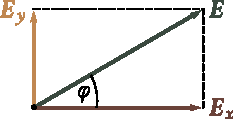
\includegraphics[scale=1]{figures/ch_19/fig_19_1.pdf}
			% \caption[]{}
            \caption[]{The resultant field strength $\vec{E}$ is the vector sum of the strengths $\vec{E}_x$ and $\vec{E}_y$.}
			\label{fig:19_1}
		\end{center}
	\end{minipage}
	\hfill{ }%space{-0.05cm}
	\begin{minipage}[t]{0.48\linewidth}
		\begin{center}
			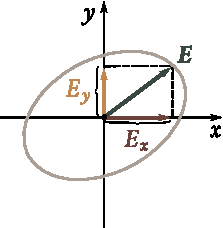
\includegraphics[scale=1]{figures/ch_19/fig_19_2.pdf}
            % \caption[]{}
			\caption[]{We consider that quantities \eqref{eq:19_1} are the coordinates of the tail of the resultant vector $\vec{E}$.}
			\label{fig:19_2}
		\end{center}
	\end{minipage}
\vspace{-0.4cm}
\end{figure}

Assume that the light waves $E_x$ and $E_y$ are coherent, with $\delta$ equal to zero or $\pi$.
Hence, according to \eqn{19_2},
\begin{equation*}
	\tan\varphi = \pm \frac{A_2}{A_1} = \text{constant}.
\end{equation*}

\noindent
Consequently, the resultant oscillation occurs in a fixed direction---the wave is plane-polarized.

When $A_1=A_2$, and $\delta=\pm\pi/2$, we have
\begin{equation*}
	\tan\varphi = \mp \tan(\omega t)
\end{equation*}

\noindent
[$\cos(\omega t\pm\pi/2) = \mp \sin(\omega t)$].
It thus follows that the plane of oscillations rotates about the direction of the ray with an angular velocity equal to the frequency of oscillation $\omega$.
The light in this case will be circularly polarized.

To find the nature of the resultant oscillation with an arbitrary constant value of $\delta$, let us take into account that quantities \eqref{eq:19_1} are the coordinates of the tail of the resultant vector $\vec{E}$ (\fig{19_2}).
We know from our treatment of oscillations (see Sec. 7.9 of Vol. I) that two mutually perpendicular harmonic oscillations of the same frequency produce motion along an ellipse when summated (in particular, motion along a straight line or a circle may be obtained).
Similarly, a point with the coordinates determined by Eqs. \eqref{eq:19_1}, \ie, the tail of vector $\vec{E}$, travels along an ellipse.
Consequently, two coherent plane-polarized light waves whose planes of oscillations are mutually
perpendicular produce an elliptically polarized light wave when superposed on each other.
At a phase difference of zero or $\pi$, the ellipse degenerates into a straight line, and plane-polarized light is obtained.
At $\delta=\pm\pi/2$ and equality of the amplitude of the waves being added, the ellipse transforms into a circle---circularly polarized light is
obtained.

Depending on the direction of rotation of the vector $\vec{E}$, right and left elliptical and circular polarizations are distinguished.
If with respect to the direction opposite that of the ray the vector $\vec{E}$ rotates clockwise, the polarization is called \textbf{right}, and in the opposite case it is \textbf{left}.

The plane in which the light vector oscillates in a plane-polarized wave will be called the \textbf{plane of oscillations}.
For historical reasons, the term \textbf{plane of polarization} was applied not to the plane in which the vector $\vec{E}$ oscillates, but to the plane perpendicular to it.

Plane-polarized light can be obtained from natural light with the aid of devices called \textbf{polarizers}.
These devices freely transmit oscillations parallel to the plane which we shall call the \textbf{polarizer plane} and completely or partly retain the oscillations perpendicular to this plane.
We shall apply the adjective \textbf{imperfect} to a polarizer that only partly retains oscillations perpendicular to its plane.
We shall apply the term ``polarizer'' for brevity to a perfect polarizer that completely retains the oscillations perpendicular to its plane and does not weaken the oscillations parallel to its plane.

Light is produced at the outlet from an imperfect polarizer in which the oscillations in one direction predominate over the oscillations in other directions.
Such light is called \textbf{partly polarized}.
It can be considered as a mixture of natural and plane-polarized light.
Partly polarized light, like natural light, can be represented in the form of a superposition of two incoherent plane-polarized waves with mutually perpendicular planes of oscillations.
The difference is that for natural light the intensity of these waves is the same, and for partly polarized light it is different.

If we pass partly polarized light through a polarizer, then when the device rotates about the direction of the ray, the intensity of the transmitted light will change within the limits from $\ab{I}{max}$ to $\ab{I}{min}$.
The transition from one of these values to the other one will occur upon rotation through an angle of $\pi/2$ (during one complete revolution both the maximum and the minimum intensity will be
reached twice).
The expression
\begin{equation}\label{eq:19_3}
	P = \frac{\ab{I}{max} - \ab{I}{min}}{\ab{I}{max} + \ab{I}{min}}
\end{equation}

\noindent
is known as the \textbf{degree of polarization}.
For plane-polarized light, $\ab{I}{min}=0$, and $P=1$.
For natural light, $\ab{I}{min}=\ab{I}{max}$ and $P=0$.

The concept of the degree of polarization cannot be applied to elliptically polarized light (in such light the oscillations are completely ordered, so that the degree of polarization always equals unity).

An oscillation of amplitude $A$ occurring in a plane making the angle $\varphi$ with the polarizer plane can be resolved into two oscillations having the amplitudes $A_{\parallel} =A\cos\varphi$ and $A_{\perp}=A\sin\varphi$ (\fig{19_3}; the ray is perpendicular to the plane of the drawing).
The first oscillation will pass through the device, the second will be retained.
The intensity of the transmitted wave is proportional to $A_{\parallel}^2= A^2 \cos^2\varphi$, \ie, is $I\cos^2\varphi$, where $I$ is the intensity of the oscillation of amplitude $A$.
Consequently, an oscillation parallel to the plane of the polarizer carries along a fraction of the intensity equal to $\cos^2\varphi$.
In natural light, all the values of $\varphi$ are equally probable.
Therefore, the fraction of the light transmitted through the polarizer will equal the average value of $\cos^2\varphi$, \ie, one-half.
When the polarizer is rotated about the direction of a natural ray, the intensity of the transmitted light remains the same.
What changes is only the orientation of the plane of oscillations of the light leaving the
device.

\begin{figure}[t]
	\begin{minipage}[t]{0.48\linewidth}
		\begin{center}
			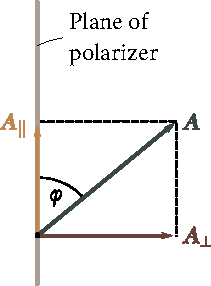
\includegraphics[scale=0.95]{figures/ch_19/fig_19_3.pdf}
			% \caption[]{}
            \caption[]{An oscillation of amplitude $A$ occurring in a plane making the angle $\varphi$ with the polarizer plane can be resolved into two oscillations having the amplitudes parallel and perpendicular: $A_{\parallel} =A\cos\varphi$ and $A_{\perp}=A\sin\varphi$.}
			\label{fig:19_3}
		\end{center}
	\end{minipage}
	\hfill{ }%space{-0.05cm}
	\begin{minipage}[t]{0.48\linewidth}
		\begin{center}
			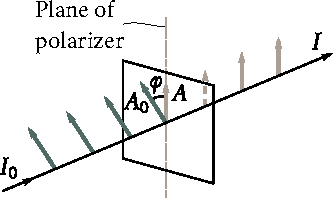
\includegraphics[scale=0.95]{figures/ch_19/fig_19_4.pdf}
            % \caption[]{}
			\caption[]{Plane-polarized light of amplitude $A_0$ and intensity $I_0$ falling on a polarizer. $\varphi$ is the angle between the plane of oscillations of the incident light and the plane of the polarizer. The component of the oscillation having the amplitude $A=A_0\cos\varphi$, will pass through the device.}
			\label{fig:19_4}
		\end{center}
	\end{minipage}
\vspace{-0.5cm}
\end{figure}

Assume that plane-polarized light of amplitude $A_0$ and intensity $I_0$ falls on a polarizer (\fig{19_4}).
The component of the oscillation having the amplitude $A=A_0\cos\varphi$, where $\varphi$ is the angle between the plane of oscillations of the incident light and the plane of the polarizer, will pass through the device.
Hence, the intensity of the transmitted light $I$ is determined by the expression
\begin{equation}\label{eq:19_4}
	I = I_0 \cos^2\varphi.
\end{equation}

\noindent
Relation \eqref{eq:19_4} is known as \textbf{Malus's law}.
It was first formulated by the French physicist Etienne Malus (1775-1812).

Let us put two polarizers whose planes make the angle $\varphi$ in the path of a natural ray.
Plane-polarized light whose intensity $I_0$ is half that of natural light will emerge from the first polarizer.
According to Malus's law, light having an intensity of $I_0\cos^2\varphi$ will emerge from the second polarizer.
The intensity of the light transmitted through both polarizers is
\begin{equation}\label{eq:19_5}
	I = \frac{1}{2} \ab{I}{nat} \cos^2\varphi.
\end{equation}

\noindent
The maximum intensity equal to $\ab{I}{nat}/2$ is obtained at $\varphi=0$ (the polarizers are parallel).
At $\varphi=\pi/2$, the intensity is zero-crossed
polarizers transmit no light.

Assume that elliptically polarized light falls on a polarizer.
The device transmits the component $\vec{E}_{\parallel}$ of the vector $\vec{E}$ in the direction of the plane of the polarizer (\fig{19_5}).
The maximum value of this component is reached at points $1$ and $2$.
Hence, the amplitude of the plane-polarized light leaving the device equals the length of $01'$.
Rotating the polarizer around the direction of the ray, we shall observe changes in the intensity ranging from $\ab{I}{max}$ (obtained when the plane of the polarizer coincides with the semimajor axis of the ellipse) to $\ab{I}{min}$ (obtained when the plane of the polarizer coincides with the semiminor axis of the ellipse).
The intensity of light for partly polarized light will change in the same way upon rotation of the polarizer.
For circularly polarized light, rotation of the polarizer is not attended (as for natural light) by a change in the intensity of the light transmitted through the device.

\begin{figure}[t]
	\begin{center}
		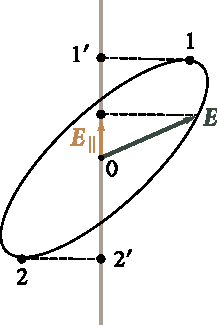
\includegraphics[scale=0.9]{figures/ch_19/fig_19_5.pdf}
		% \caption[]{}
        \caption[]{For elliptically polarized light falling on a polarizer, the device transmits the component $\vec{E}_{\parallel}$ of the vector $\vec{E}$ in the direction of the plane of the polarizer. The maximum value of this component is reached at points $1$ and $2$.}
		\label{fig:19_5}
	\end{center}
	\vspace{-0.8cm}
\end{figure}

\section{Polarization in Reflection and Refraction}\label{sec:19_2}

If the angle of incidence of light on the interface between two dielectrics (for example, on the surface of a glass plate) differs from
zero, the reflected and refracted rays will be partly polarized\footnote{Elliptically polarized light is obtained upon reflection from a conducting surface (for example, from the surface of a metal).}.
Oscillations perpendicular to the plane of incidence predominate in the reflected ray (in \fig{19_6} these oscillations are denoted by points), and oscillations parallel to the plane of incidence predominate in the refracted ray (they are depicted in the figure by double-headed arrows).
The degree of polarization depends on the
angle of incidence.
Let $\ab{\theta}{Br}$ stand for the angle satisfying the condition
\vspace{-12pt}
\begin{equation}\label{eq:19_6}
	\tan\ab{\theta}{Br} = n_{12}
\end{equation}

\noindent
($n_{12}$ is the refractive index of the second
medium relative to the first one).
At an angle of incidence $\theta_1$ equal to $\ab{\theta}{Br}$, the \fig{19_6} reflected ray is completely polarized (it contains only oscillations perpendicular to the plane of incidence).
The degree of polarization of the refracted ray at an angle of incidence equal to $\ab{\theta}{Br}$ reaches its maximum value, but this ray remains polarized only partly.

\begin{figure}[t]
	\begin{center}
		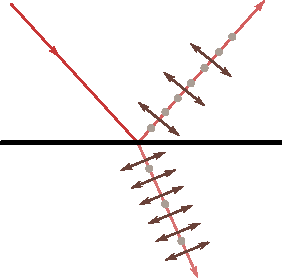
\includegraphics[scale=0.85]{figures/ch_19/fig_19_6.pdf}
		% \caption[]{}
        \caption[]{Polarization in reflection and refraction. Oscillations perpendicular to the plane of incidence predominate in the reflected ray (dots) and oscillations parallel to the plane of incidence predominate in the refracted ray (double-headed arrows).}
		\label{fig:19_6}
	\end{center}
	\vspace{-1cm}
\end{figure}

Relation \eqref{eq:19_6} is known as \textbf{Brewster's law}, in honour to its discoverer, the British physicist David Brewster (1781-1868), and the angle $\ab{\theta}{Br}$ is called \textbf{Brewster's angle}.
It is easy to see that when light falls at Brewster's angle, the reflected and refracted rays are mutually perpendicular.
The degree of polarization of the reflected and refracted rays for different angles of incidence can be obtained with the aid of Fresnel's formulas.
The latter follow from the conditions imposed on an electromagnetic field at the interface between two dielectrics\footnote{Fresnel obtained these formulas on the basis of the notions of light as of elastic waves propagating in ether.}.
These conditions include the equality of the tangential components of the vectors $\vec{E}$ and $\vec{H}$, and also the equality of the normal components of the vectors $\vec{D}$ and $\vec{B}$ at both sides of the interface (for one
side the sum of the relevant vectors for the incident and reflected waves must be taken, and for the other, the vector for the refracted
wave).

Fresnel's formulas establish the relations between the complex amplitudes of the incident, reflected, and refracted waves.
We remind our reader that by the complex amplitude $\hat{A}$ is meant the expression $Ae^{i\alpha}$, where $A$ is the conventional amplitude, and $\alpha$ is the initial phase of the oscillations.
Hence, the equality of two complex amplitudes signifies the equality of both the conventional amplitudes and the initial phases of the two oscillations:
\begin{equation}\label{eq:19_7}
	\hat{A}_1 = \hat{A}_2 \Rightarrow A_1=A_2 \text{ and } \alpha_1=\alpha_2.
\end{equation}

\noindent
When the complex amplitudes differ in sign, the conventional ones are the same, while the initial phases differ by $\pi$ ($e^{i\pi}=-1$):
\begin{equation}\label{eq:19_8}
	\hat{A}_1 = -\hat{A}_2 \Rightarrow A_1=A_2 \text{ and } \alpha_1=\alpha_2+\pi.
\end{equation}

Let us represent the incident wave in the form of a superposition of two incoherent waves in one of which the oscillations occur in the plane of incidence, and in the other, are perpendicular to this plane.
Let us denote the complex amplitude of the first wave by $\hat{A}_{\parallel}$, and of the second by $\hat{A}_{\perp}$.
We shall proceed similarly with the reflected and refracted waves.
We shall use the same symbols for the amplitudes of the reflected waves, adding one prime, and the
same symbols for the amplitudes of the refracted waves, adding two primes.
Thus,
\begin{itemize}[]
	\item $\hat{A}_{\parallel}$ and $\hat{A}_{\perp} = $ amplitudes of the incident waves,
	\item $\hat{A}_{\parallel}'$ and $\hat{A}_{\perp}' = $ amplitudes of the reflected waves,
	\item $\hat{A}_{\parallel}''$ and $\hat{A}_{\perp}'' = $ amplitudes of the refracted waves.
\end{itemize}

Fresnel's formulas have the following form\footnote{Fresnel's formulas are customarily written without ``caps'' over the amplitudes. To underline the fact that we are dealing with complex amplitudes, however, we found it helpful to write the amplitudes with the ``caps''.}:
\begin{equation}\label{eq:19_9}
	\begin{cases}
		&\!\!\! \hat{A}_{\parallel}' = \hat{A}_{\parallel} \dfrac{\tan(\theta_1-\theta_2)}{\tan(\theta_1+\theta_2)},\quad
		\hat{A}_{\perp}' = \hat{A}_{\perp} \dfrac{\sin(\theta_1-\theta_2)}{\sin(\theta_1+\theta_2)}\\[8pt]
		&\!\!\! \hat{A}_{\parallel}'' = \hat{A}_{\parallel} \dfrac{2\sin\theta_2\cos\theta_1}{\sin(\theta_1+\theta_2)\cos(\theta_1-\theta_2)},\quad \hat{A}_{\perp}'' = \hat{A}_{\perp} \dfrac{2\sin\theta_2\cos\theta_1}{\sin(\theta_1+\theta_2)}
	\end{cases}
\end{equation}

\noindent
($\theta_1$ is the angle of incidence, and $\theta_2$ is the angle of refraction of the light wave).
We must underline the fact that formulas \eqref{eq:19_9} establish the relations between the complex amplitudes at the interface between dielectrics, \ie, at the point of incidence of a ray on this interface.

It can be seen from the last two of formulas \eqref{eq:19_9} that the signs of the complex amplitudes of the incident and refracted waves at any values of the angles $\theta_1$ and $\theta_2$ are the same (the sum of $\theta_1$ and $\theta_2$ cannot exceed $\pi$).
This signifies that when penetrating into the second medium, the phase of the wave does not undergo a jump.
In dealing with the phase relations between an incident and a reflected wave, we must take into account that for a wave polarized perpendicularly to the plane of incidence, the coincidence of the
signs of $\hat{A}_{\perp}$ and $\hat{A}_{\perp}'$ corresponds to the absence of a jump in the phase in reflection (\fig{19_7}a).
For a wave that is polarized in the plane of incidence, on the other hand, a jump in the phase is absent when the signs of $\hat{A}_{\parallel}$ and $\hat{A}_{\parallel}'$ are opposite (\fig{19_7}b).

\begin{figure}[t]
	\begin{center}
		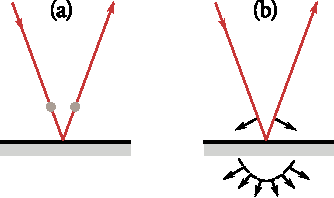
\includegraphics[scale=1]{figures/ch_19/fig_19_7.pdf}
		% \caption[]{}
        \caption[]{Dealing with phase relations. (a) For a wave polarized perpendicularly to the plane of incidence, the coincidence of the signs of $\hat{A}_{\perp}$ and $\hat{A}_{\perp}'$ corresponds to the absence of a jump in the phase in reflection. (b) For a wave that is polarized in the plane of incidence, on the other hand, a jump in the phase is absent when the signs of $\hat{A}_{\parallel}$ and $\hat{A}_{\parallel}'$ are opposite.}
		\label{fig:19_7}
	\end{center}
	\vspace{-0.8cm}
\end{figure}

The phase relations between the reflected and incident waves depend on the relation between the refractive indices $n_1$ and $n_2$ of the first and second media, and also on the relation between the angle of incidence $\theta_1$ and Brewster's angle $\ab{\theta}{Br}$ (we remind our reader that when $\theta_1 = \ab{\theta}{Br}$, the sum of the angles $\theta_1$ and $\theta_2$, is $\pi/2$).
Table \ref{table:19_1} gives the results following from the first two of formulas \eqref{eq:19_9} in
four possible cases.
It follows from the table that for incidence at an angle less than Brewster's angle, reflection from an optically denser medium is attended by a jump in phase of $\pi$; reflection from an optically less dense medium occurs without a change in phase.
This result for $\theta_1=0$ was obtained in \sect{16_3}.
When $\theta_1>\ab{\theta}{Br}$, the phase relations for both wave components are different.

We obtain from the first of formulas \eqref{eq:19_9} that when $\theta_1+\theta_2=\pi/2$, \ie, at $\theta_1=\ab{\theta}{Br}$, the amplitude $\hat{A}_{\parallel}'$ vanishes.
Consequently, only oscillations perpendicular to the plane of incidence are present in the reflected wave---the latter is completely polarized.
Thus, \textit{Brewster's law directly follows from Fresnel's formulas}.

\begin{table}[!b]
	\renewcommand{\arraystretch}{1.2}
	\caption{}
	\vspace{-0.6cm}
	\label{table:19_1}
	\begin{center}\resizebox{0.9\linewidth}{!}{
			\begin{tabular}{p{1.3cm} p{4.5cm} p{4.5cm}}
				\toprule[1pt]
				 & $\theta_1<\ab{\theta}{Br}\, (\theta_1+\theta_2<\pi/2)$ & $\theta_1>\ab{\theta}{Br}\, (\theta_1+\theta_2>\pi/2)$\\
				\midrule[0.5pt]\midrule[0.5pt]
				$n_2>n_1$, $\theta_1>\theta_2$ & The signs of $\hat{A}_{\parallel}'$ and $\hat{A}_{\parallel}$ are the same (a phase jump by $\pi$).

				The sign of $\hat{A}_{\perp}'$ is opposite to that of $\hat{A}_{\perp}'$ (a phase jump by $\pi$). & The sign of $\hat{A}_{\parallel}'$ is opposite to that of $\hat{A}_{\parallel}$ (no phase jump).

				The sign of $\hat{A}_{\perp}'$ is opposite to that of $\hat{A}_{\parallel}$ (a phase jump by $\pi$).\\
				\midrule[0.5pt]
				$n_2<n_1$, $\theta_1<\theta_2$ & The sign of $\hat{A}_{\parallel}'$ is opposite to that of $\hat{A}_{\parallel}$ (no phase jump).

				The signs of $\hat{A}_{\perp}'$ and $\hat{A}_{\perp}'$ are the same (no phase jump). & The signs of $\hat{A}_{\parallel}'$ and $\hat{A}_{\parallel}$ are the same (a phase jump by $\pi$).

				The signs of $\hat{A}_{\perp}'$ and $\hat{A}_{\perp}$ are the same (no phase jump).\\
				\bottomrule[1pt]
			\end{tabular}
	}\end{center}
\end{table}

At small angles of incidence, the sines and tangents in formulas \eqref{eq:19_9} may be replaced by the angles themselves, and the cosines
may be assumed equal to unity.
In addition, in this case we may consider that $\theta_1=n_{12}\theta_2$ (this follows from the law of refraction after the sines are replaced with the relevant angles).
As a result, Fresnel's formulas for small angles of incidence acquire the form
\begin{equation}\label{eq:19_10}
	\text{small }\theta_1 \Rightarrow \begin{cases}
		&\!\!\! \hat{A}_{\parallel}' = \hat{A}_{\parallel} \dfrac{\theta_1-\theta_2}{\theta_1+\theta_2} = \hat{A}_{\parallel} \dfrac{n_{12}-1}{n_{12}+1}\\[8pt]
		&\!\!\! \hat{A}_{\perp}' = \hat{A}_{\perp} \dfrac{\theta_1-\theta_2}{\theta_1+\theta_2} = - \hat{A}_{\perp} \dfrac{n_{12}-1}{n_{12}+1}\\[8pt]
		&\!\!\! \hat{A}_{\parallel}'' = \hat{A}_{\parallel} \dfrac{2\theta_2}{\theta_1+\theta_2} = \hat{A}_{\parallel} \dfrac{2}{n_{12}+1}\\[8pt]
		&\!\!\! \hat{A}_{\perp}'' = \hat{A}_{\perp} \dfrac{2\theta_2}{\theta_1+\theta_2} = \hat{A}_{\perp} \dfrac{2}{n_{12}+1}.
	\end{cases}
\end{equation}

Squaring Eqs. \eqref{eq:19_10} and multiplying the expressions obtained by the refractive index of the relevant medium, we get relations between the intensities of the incident, reflected, and refracted rays for small angles of incidence [see expression \eqref{eq:19_6}].
Here, for example, the intensity of the reflected light $I'$ can be calculated as the sum of the intensities of both components $I_{\parallel}'$ and $I_{\perp}'$ because these components are not coherent in natural light [the intensities instead of the amplitudes are summated for incoherent waves, see \eqn{17_1}].
As a result, we get
\begin{equation*}
	I' = I \parenthesis{\frac{n_{12}-1}{n_{12}+1}}^2, \quad
\end{equation*}

\noindent
From these formulas, we get \eqns{16_33}{16_34} for $\rho$ and $\tau$.

\section{Polarization in Double Refraction}\label{sec:19_3}

When light passes through all transparent crystals except for those belonging to the cubic system, a phenomenon is observed called \textbf{double refraction}\footnote{Double refraction was first observed in 1669 by the Danish scientist Erasm Bartholin (1625-1698) for Iceland spar (a variety of calcium carbonate \ce{CaCO3}---crystals of the hexagonal system).}.
It consists in that a ray falling on a crystal is split inside the latter into two rays propagating, generally speaking, with different velocities and in different directions.

Doubly refracting (or birefringent) crystals are divided into \textbf{uniaxial} and \textbf{biaxial} ones.
In uniaxial crystals, one of the refracted rays obeys the conventional law of refraction, in particular, it is in the same plane as the incident ray and a normal to the refracting surface.
This ray is called an \textbf{ordinary ray} and is designated by the symbol o.
For the other ray, called an \textbf{extraordinary ray} (designated by e), the ratio of the sines of the angle of incidence and the angle of refraction does not remain constant when the angle of incidence varies.
Even upon normal incidence of light \fig{19_8} on a crystal, an extraordinary ray, generally speaking, deviates from a normal (\fig{19_8}).
In addition, an extraordinary ray does not lie, as a rule, in the same plane as the incident ray and a normal to the refracting surface.
Examples of uniaxial crystals are Iceland spar, quartz, and tourmaline.
In biaxial crystals (mica, gypsum), both rays are extraordinary---the refractive indices for them depend on the direction in the crystal.
In the following, we shall be concerned only with uniaxial crystals.

\begin{figure}[t]
	\begin{center}
		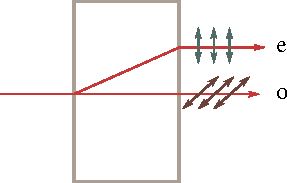
\includegraphics[scale=1]{figures/ch_19/fig_19_8.pdf}
		% \caption[]{}
        \caption[]{Double refraction or birefringence. Doubly refracting (or birefringent) crystals are divided into uniaxial and biaxial ones. In uniaxial crystals, one of the refracted rays (ordinary rays ``o'') obeys the conventional law of refraction, in particular it is in the same plane as the incident ray and a normal to the refracting surface, while the extraordinary ray (``e'') deviates from a normal.}
		\label{fig:19_8}
	\end{center}
	\vspace{-0.8cm}
\end{figure}

Uniaxial crystals have a direction along which ordinary and extraordinary rays propagate without separation and with the same velocity\footnote{Biaxial crystals have two such directions.}.
This direction is known as the \textbf{optical axis} of the crystal.
It must be borne in mind that an optical axis is not a straight line passing through a point of a crystal, but a definite direction in the crystal.
Any straight line parallel to the given direction is an optical axis of the crystal.

A plane passing through an optical axis is called a \textbf{principal section} or a \textbf{principal plane} of the crystal. Customarily, the principal section passing through the light ray is used.

Investigation of the ordinary and extraordinary rays shows that they are both completely polarized in mutually perpendicular directions
(see \fig{19_8}).
The plane of oscillations of the ordinary ray is perpendicular to a principal section of the crystal.
In the extraordinary ray, the oscillations of the light vector occur in a plane coinciding with a principal section.
When they emerge from the crystal, the two rays differ from each other only in the direction of polarization so that the terms ``ordinary'' and ``extraordinary'' have a meaning only inside the crystal.

In some crystals, one of the rays is absorbed to a greater extent than the other.
This phenomenon is called \textbf{dichroism}.
A crystal of tourmaline (a mineral of a complex composition) displays very great dichroism in visible rays.
An ordinary ray is virtually completely absorbed
in it over a distance of \SI{1}{\milli\metre}.
In crystals of iodoquinine sulphate, one of the rays is absorbed over a path of about \SI{0.1}{\milli\metre}.
This circumstance has been taken advantage of for manufacturing a polarizing device called a \textbf{polaroid}.
It is a celluloid film into which a great number of identically oriented minute crystals of iodoquinine sulphate have been introduced.

Double refraction is explained by the anisotropy
of crystals.
In crystals of the noncubic system, the permittivity $\varepsilon$ depends on the direction.
In uniaxial crystals, $\varepsilon$ in the direction of an optical axis and in directions perpendicular to it has different values $\varepsilon_{\parallel}$ and $\varepsilon_{\perp}$.
In other directions, $\varepsilon$ has intermediate values.
According to \eqn{16_3} $n=\sqrt{\varepsilon}$.
It thus follows from the anisotropy of $\varepsilon$, that \textit{different values of the refractive index $n$ correspond to electromagnetic waves with different directions of the oscillations of the vector $\vec{E}$}.
Therefore, the velocity of the light waves depends on the direction of oscillations of the light vector $\vec{E}$.

\begin{figure}[t]
	\begin{center}
		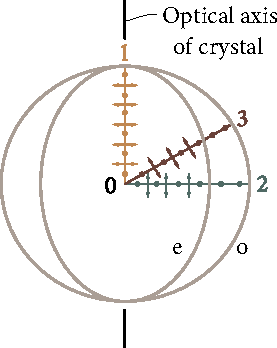
\includegraphics[scale=0.95]{figures/ch_19/fig_19_9.pdf}
		% \caption[]{}
        \caption[]{In an ordinary ray, the oscillations of the light vector occur in a direction perpendicular to a principal section of the crystal (depicted by dots on the relevant ray). The oscillations in an extraordinary ray take place in a principal section. The directions of oscillations of the vector $\vec{E}$ are depicted by double-headed arrows, making different angles a with an optical axis.}
		\label{fig:19_9}
	\end{center}
	\vspace{-0.8cm}
\end{figure}

In an ordinary ray, the oscillations of the light vector occur in a direction perpendicular to a principal section of the crystal (in \fig{19_9} these oscillations are depicted by dots on the relevant ray).
Therefore, with any direction of an ordinary ray (three directions $1$, $2$, and $3$ are shown in the figure), the vector $\vec{E}$ makes a right angle with an optical axis of the crystal, and the velocity of the light wave will be the same, equal to $\ab{v}{o}=c/\sqrt{\varepsilon_{\perp}}$.
Depicting the velocity of an ordinary ray in the form of lengths laid off in different directions,
we shall get a spherical surface.
Figure \ref{fig:19_9} shows the intersection of this surface with the plane of the drawing.
A picture such as that in \fig{19_9} is observed in any principal section, \ie, in any plane passing through an optical axis.
Let us imagine that a point source of light is placed at point $0$ inside a crystal.
Hence, the sphere which we have constructed will be the wave surface of ordinary rays.

The oscillations in an extraordinary ray take place in a principal section.
Therefore, for different rays, the directions of oscillations of the vector $\vec{E}$ (in \fig{19_9} these directions are depicted by double-headed arrows) make different angles a with an optical axis.
For ray $1$, the angle $\alpha$ is $\pi/2$, owing to which the velocity is $\ab{v}{o}=c/\sqrt{\varepsilon_{\perp}}$, for ray $2$, the angle $\alpha=0$, and the velocity is $\ab{v}{e}= c/\sqrt{\varepsilon_{\parallel}}$.
For ray $3$, the velocity has an intermediate value.
We can show that the wave surface of extraordinary rays is an ellipsoid of revolution.
At places of intersection with an optical axis of the crystal, this ellipsoid and the sphere constructed for the ordinary rays come into contact.

Uniaxial crystals are characterized by a \textbf{refractive index of an ordinary ray} equal to $\ab{n}{o}=c/\ab{v}{o}$, and a refractive index of an extraordinary ray perpendicular to an optical axis equal to $\ab{n}{e}=c/\ab{v}{e}$.
The latter quantity is called simply the \textbf{refractive index of an extraordinary
ray}.

Depending on which of the velocities, $\ab{v}{o}$ or $\ab{v}{e}$, is greater, \textbf{positive} and \textbf{negative} uniaxial crystals are distinguished (\fig{19_10}).
For positive crystals, $\ab{v}{e}<\ab{v}{o}$ (this means that $\ab{n}{e}>\ab{n}{o}$).
For negative crystals, $\ab{v}{e}>\ab{v}{o}$ ($\ab{n}{e}<\ab{n}{o}$).
It is simple to remember what crystals are called positive and what negative.
For positive crystals, the ellipsoid of velocities is extended along an optical axis reminding one of the vertical line in the sign ``+''; for negative crystals, the ellipsoid of velocities is extended in a direction perpendicular to an optical axis, reminding one of the sign ``-''.

\begin{figure}[t]
	\begin{minipage}[t]{0.56\linewidth}
		\begin{center}
			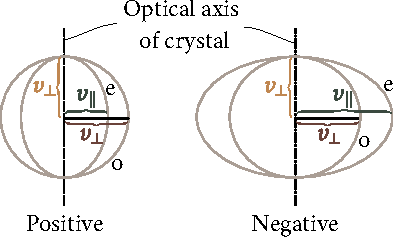
\includegraphics[scale=1]{figures/ch_19/fig_19_10.pdf}
			% \caption[]{}
            \caption[]{Depending on which of the velocities, $\ab{v}{o}$ or $\ab{v}{e}$, is greater, positive and negative uniaxial crystals are distinguished. Positive crystals, $\ab{v}{e}<\ab{v}{o}$ ($\ab{n}{e}>\ab{n}{o}$);
			negative crystals, $\ab{v}{e}>\ab{v}{o}$ ($\ab{n}{e}<\ab{n}{o}$).}
			\label{fig:19_10}
		\end{center}
	\end{minipage}
	\hfill{ }%space{-0.05cm}
	\begin{minipage}[t]{0.4\linewidth}
		\begin{center}
			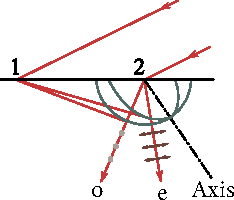
\includegraphics[scale=1]{figures/ch_19/fig_19_11.pdf}
            % \caption[]{}
			\caption[]{Wave surfaces of an ordinary and extraordinary rays with their centre at point $2$ on the surface of the crystal.}
			\label{fig:19_11}
		\end{center}
	\end{minipage}
\vspace{-0.4cm}
\end{figure}

The path of an ordinary and an extraordinary ray in a crystal can be determined with the aid of the Huygens principle.
Figure \ref{fig:19_11} depicts wave surfaces of an ordinary and extraordinary rays with their centre at point $2$ on the surface of the crystal.
The construction is for the moment of time when the wavefront of the incident wave reaches point $1$.
The envelopes of all the secondary wavelets (the waves whose centres are in the interval between points $1$ and $2$ are not shown in the figure) for the ordinary and extraordinary rays are evidently planes.
The refracted ray o or e emerging from point $2$ passes through the point of contact of the envelope with the relevant wave surface.

We remind our reader that rays are defined as lines along which the energy of a light wave
propagates (see \sect{16_1}).
A glance at \fig{19_11} shows that the ordinary ray o coincides with a normal to the relevant wave
surface.
The extraordinary ray e, on the other hand, appreciably deviates from a normal to the wave surface.

Figure \ref{fig:19_12} shows three cases of the normal incidence of light on the surface of a crystal differing in the direction of the optical
axis.
In case (a), the rays o and e propagate along an optical axis and therefore travel without separating.
Inspection of \fig{19_12}b shows that even upon normal incidence of light on a refracting surface, an extraordinary ray may deviate from a normal to this surface (compare with \fig{19_8}).
In \fig{19_12}c, the optical axis of the crystal is parallel to the refracting surface.
In this case with normal incidence of the light, the ordinary and extraordinary rays travel in the same direction, but propagate with different velocities.
The result is a constantly growing phase difference between them.
The nature of polarization of the ordinary and extraordinary rays in \fig{19_12} is not indicated.
It is the same as for the rays depicted in \fig{19_11}.

\begin{figure}[t]
	\begin{center}
		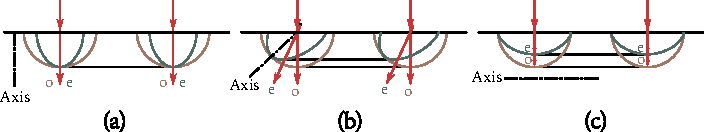
\includegraphics[scale=0.95]{figures/ch_19/fig_19_12h.pdf}
		% \caption[]{}
        \caption[]{Three cases of the normal incidence of light on the surface of a crystal differing in the direction of the optical axis. (a) The rays o and e propagate along an optical axis without separating. (b) An extraordinary ray may deviate from a normal to this surface. (c) The ordinary and extraordinary rays travel in the same direction, but propagate with different velocities.}
		\label{fig:19_12}
	\end{center}
	\vspace{-0.8cm}
\end{figure}

\section{Interference of Polarized Rays}\label{sec:19_4}

When two coherent rays polarized in mutually perpendicular directions are superposed, no interference pattern with the characteristic alternation of maxima and minima of the intensity can be obtained.
Interference occurs only when the oscillations in the interacting rays occur along the same direction.
The oscillations in two rays initially polarized in mutually perpendicular directions can be brought into one plane by passing these rays through a polarizer installed so that its plane does not coincide with the plane of oscillations
of any of the rays.

Let us see what happens when an ordinary and an extraordinary ray emerging from a crystal plate are superposed.
Assume that the plate has been cut out parallel to an optical axis (\fig{19_13}).
With normal incidence of the light on the plate, the ordinary and extraordinary rays will propagate without separating, but with different velocities (see \fig{19_12}c).
The following path difference appears between the rays while they pass through the plate:
\begin{equation}\label{eq:19_11}
	\Delta = (\ab{n}{o} - \ab{n}{e}) d,
\end{equation}

\noindent
or the following phase difference:
\begin{equation}\label{eq:19_12}
	\delta = \frac{(\ab{n}{o} - \ab{n}{e}) d}{\lambda_0} 2\pi
\end{equation}

\noindent
($d$ is the plate thickness, and $\lambda_0$ the wavelength in a vacuum).

\begin{figure}[t]
	\begin{center}
		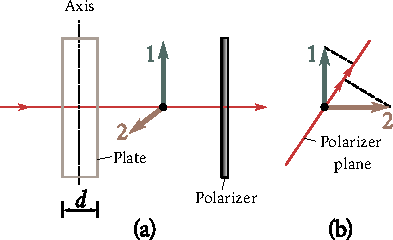
\includegraphics[scale=1]{figures/ch_19/fig_19_13.pdf}
		% \caption[]{}
        \caption[]{Superposed ordinary and an extraordinary ray emerging from a crystal plate. (a) Light through a crystal plate cut out parallel to the optical axis. Rays $1$ and $2$ that are polarized in mutually perpendicular planes will emerge from the plate. (b) With a polarizer in the path of these rays, both rays will oscillate in one plane (polarizer plane) after passing through the polarizer.}
		\label{fig:19_13}
	\end{center}
	\vspace{-0.8cm}
\end{figure}

Thus, if we pass natural light through a crystal plate cut out parallel to the optical axis (\fig{19_13}a), two rays $1$ and $2$ that are
polarized in mutually perpendicular planes will emerge from the plate\footnote{In the crystal, ray $1$ was extraordinary and could be designated by the symbol e, and ray $2$ was ordinary (o). Upon emerging from the crystal, these rays lost their right to be called ordinary and extraordinary.}, and between them there will be a phase difference determined by \eqn{19_12}.
Let us place a polarizer in the path of these rays.
Both rays after passing through the polarizer will oscillate in one plane.
Their amplitudes will equal the components of the amplitudes of rays $1$ and $2$ in the direction of the plane of the polarizer (\fig{19_13}b).

The rays emerging from the polarizer are produced as a result of division of the light obtained from a single source.
Therefore, they ought to interfere.
If rays $1$ and $2$ are produced as a result of natural light passing through the plate, however, they do not interfere.
The explanation is very simple.
Although the ordinary and extraordinary rays are produced by the same light source, they contain mainly oscillations belonging to different wave trains emitted by individual atoms.
The oscillations in the ordinary ray are predominantly due to the trains whose oscillation planes are close to one direction in space, whereas those in the extraordinary ray are due to trains whose oscillation planes are close to another direction perpendicular to the first one.
Since the individual trains are incoherent, the ordinary and extraordinary rays produced from natural light, and, consequently, rays $1$ and $2$ too, are also incoherent.

Matters are different if plane-polarized light falls on a crystal plate.
In this case, the oscillations of each train are divided between the ordinary and extraordinary rays in the same proportion (depending on the orientation of an optical axis of the plate relative to the plane of oscillations in the incident ray).
Consequently, rays o and e, and therefore rays $1$ and $2$ too, will be coherent and will interfere.

\section{Passing of Plane-Polarized Light Through a Crystal Plate}\label{sec:19_5}

Let us consider a crystal plate cut out parallel to an optical axis.
We saw in the preceding section that when plane-polarized light falls on such a plate, the ordinary and extraordinary rays are coherent.
At the entrance to the plate, the phase difference $\delta$ of these rays is zero, and at the exit from the plate
\begin{equation}\label{eq:19_13}
	\delta = \frac{\Delta}{\lambda_0} 2\pi = \frac{(\ab{n}{o} - \ab{n}{e}) d}{\lambda_0} 2\pi
\end{equation}

\noindent
[see \eqns{19_11}{19_12}; we assume that the light falls on the plate normally].

A plate cut out parallel to an optical axis for which
\begin{equation*}
	(\ab{n}{o} - \ab{n}{e}) d = m\lambda_0 + \frac{\lambda_0}{4}
\end{equation*}

\noindent
($m$ is any integer or zero) is called a \textbf{quarter-wave plate}.
An ordinary and an extraordinary rays passing through such a plate acquire a phase difference equal to $\pi/2$ (we remind our reader that the phase difference is determined with an accuracy to $2\pi m$).
A plate for which
\begin{equation*}
	(\ab{n}{o} - \ab{n}{e}) d = m\lambda_0 + \frac{\lambda_0}{2}
\end{equation*}

\noindent
is called a \textbf{half-wave plate}, etc.

Let us see how plane-polarized light passes through a half-wave plate.
The oscillation of $\vec{E}$ in the incident ray occurring in plane P produces the oscillation of $\ab{\vec{E}}{o}$ of the ordinary ray and the oscillation of $\ab{\vec{E}}{e}$ of the extraordinary ray when entering the crystal (\fig{19_14}).
During the time spent in passing through the plate, the phase difference between the oscillations of $\ab{\vec{E}}{o}$ and $\ab{\vec{E}}{e}$ changes by $\pi$.
Therefore, at the exit from the plate, the phase relation between the ordinary and extraordinary rays will correspond to the mutual arrangement
of the vectors $\ab{\vec{E}}{e}$ and $\ab{\vec{E}}{o}'$ (at the entrance to the plate it corresponded to the mutual arrangement of the vectors $\ab{\vec{E}}{e}$ and $\ab{\vec{E}}{o}$).
Consequently, the light emerging from the plate will be polarized in plane P$'$.
Planes P and P$'$ are symmetrical relative to optical axis $0$ of the plate.
Thus, a half-wave plate turns the plane of oscillations of the light passing through it through the angle $2\varphi$ ($\varphi$ is the angle between the plane of oscillations in the incident ray and the axis of the plate).

\begin{figure}[t]
	\begin{minipage}[t]{0.44\linewidth}
		\begin{center}
			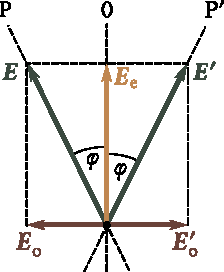
\includegraphics[scale=1]{figures/ch_19/fig_19_14.pdf}
			% \caption[]{}
            \caption[]{A half-wave plate turns the plane of oscillations of the light passing through it through the angle $2\varphi$ ($\varphi$ is the angle between the plane of oscillations in the incident ray and the axis of the plate). This means that passing through the plate the phase difference between the oscillations of $\ab{\vec{E}}{o}$ and $\ab{\vec{E}}{e}$ changes by $\pi$.}
			\label{fig:19_14}
		\end{center}
	\end{minipage}
	\hfill{ }%space{-0.05cm}
	\begin{minipage}[t]{0.52\linewidth}
		\begin{center}
			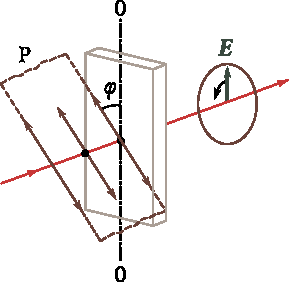
\includegraphics[scale=1]{figures/ch_19/fig_19_15.pdf}
            % \caption[]{}
			\caption[]{For a plane-polarized light through a quarter-wave plate at $\varphi=\SI{45}{\degree}$, the amplitudes of both rays emerging from the plate will be the same (no dichroism), with phase shift of $\pi/2$, and the light will be circularly polarized. At a different value of the $\varphi$, the amplitudes of the rays emerging from the plate will be different. These rays when superposed form elliptically polarized light.}
			\label{fig:19_15}
		\end{center}
	\end{minipage}
\vspace{-0.4cm}
\end{figure}

Now let us pass plane-polarized light through a quarter-wave plate (\fig{19_15}).
If we arrange the plate so that the angle $\varphi$ between plane of oscillations P in the incident ray and plate axis $0$ is \SI{45}{\degree}, the amplitudes of both rays emerging from the plate will be the same (dichroism is assumed to be absent).
The phase shift between the oscillations in these rays will be $\pi/2$.
Hence, the light emerging from the plate will be circularly polarized.
At a different value of the angle $\varphi$, the amplitudes of the rays emerging from the plate will be different.
Consequently, these rays when superposed form elliptically polarized light; one of the axes of the ellipse coincides with plate axis $0$.

When plane-polarized light is passed through a plate with a fractional number of waves not coinciding with $m+1/4$ or $m+1/2$, two coherent light waves polarized in mutually perpendicular planes will emerge from the plate.
Their phase difference is other than $\pi/2$ and other than $\pi$.
Hence, with any relation between the amplitudes of these waves depending on the angle $\varphi$ (see \fig{19_15}), elliptically polarized light will be produced at the exit from the plate, and none of the axes of the ellipse will coincide with plate axis $0$.
The orientation of the ellipse axes relative to axis $0$ is determined by the phase difference $\delta$, and also by the ratio of the amplitudes,
\ie, by the angle $\varphi$ between the plane of oscillations in the incident wave and plate axis $0$.

We must note that regardless of the plate thickness, when $\varphi$ is zero or $\pi/2$, only one ray will propagate in the plate (in the first case an extraordinary ray, in the second case an ordinary one) so that at the plate exit the light remains plane-polarized with its plane of oscillations coinciding with P.

If we place a quarter-wave plate in the path of elliptically polarized light and arrange its optical axis along one of the ellipse axes, then the plate will introduce an additional phase difference equal to $\pi/2$.
As a result, the phase difference between two plane-polarized waves whose sum is an elliptically polarized wave becomes equal to zero or $\pi$, so that the superposition of these waves produces a plane-polarized wave.
Hence, a properly turned quarter-wave plate transforms elliptically polarized light into plane-polarized light.
This underlies a method by means of which we can distinguish elliptically polarized light from partly polarized light, or circularly polarized light from natural light.
The light being studied is passed through a quarter-wave plate and a polarizer placed after it.
If the ray being studied is elliptically polarized (or circularly polarized), then by rotating the plate and the polarizer around the direction of the ray, we can achieve complete darkening of the field of vision.
If the light is partly polarized (or natural), it is impossible to achieve extinction of the ray being studied with any position of the plate and polarizer.

\section{A Crystal Plate Between Two Polarizers}\label{sec:19_6}

Let us place a plate made from a uniaxial crystal cut out parallel to optical axis $0$ between polarizers\footnote{The second polarizer P$'$ in the direction of ray propagation is also called
an analyzer.} P and P$'$ (\fig{19_16}).
Plane-polarized light of intensity $I$ will emerge from polarizer P.
In passing through the plate, the light in the general case will become elliptically polarized.
When it emerges from polarizer P$'$, the light will again be plane-polarized.
Its intensity $I'$ depends on the mutual orientation of the planes of polarizers P and P$'$ and an optical axis of the plate, and also on the phase difference $\delta$ acquired by the ordinary and extraordinary rays when they pass through the plate.

\begin{figure}[t]
	\begin{center}
		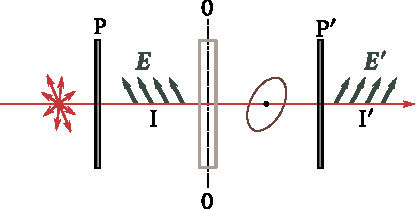
\includegraphics[scale=1]{figures/ch_19/fig_19_16.pdf}
		% \caption[]{}
        \caption[]{Plate made from a uniaxial crystal cut out parallel to optical axis $0$ between polarizers P and P$'$. Plane-polarized light of intensity $I$ will emerge from polarizer P. In passing through the plate, the light in the general case will become elliptically polarized.}
		\label{fig:19_16}
	\end{center}
	\vspace{-0.8cm}
\end{figure}

Assume that the angle $\varphi$ between the plane of polarizer P and plate axis $0$ is $\pi/4$.
Let us consider two particular cases: the polarizers are parallel (\fig{19_17}a), and they are crossed (\fig{19_17}b).
The light oscillation leaving polarizer P will be depicted by the vector $\vec{E}$ in plane P.
At the entrance to the plate, the oscillation of $\vec{E}$ will produce two oscillations---the oscillation of $\ab{\vec{E}}{o}$ (ordinary ray) perpendicular to the optical axis, and the oscillation of $\ab{\vec{E}}{e}$ (extraordinary ray) parallel to the axis.
These oscillations will be coherent; in passing through the plate, they acquire the phase difference $\delta$ that is determined by the plate thickness and the difference between the refractive indices of the ordinary and extraordinary rays.
The amplitudes of these oscillations are the same and equal
\begin{equation}\label{eq:19_14}
	\ab{E}{o} = \ab{E}{e} = E \cos\parenthesis{\frac{\pi}{4}} = \frac{E}{\sqrt{2}},
\end{equation}

\noindent
where $E$ is the amplitude of the wave emerging from the first polarizer.

\begin{figure}[t]
	\begin{center}
		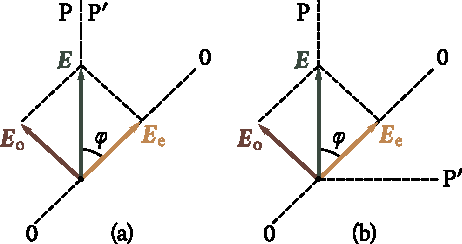
\includegraphics[scale=1]{figures/ch_19/fig_19_17.pdf}
		% \caption[]{}
        \caption[]{Two particular cases for when the polarizers are parallel (a) and when are crossed (b). The light oscillation leaving polarizer P will be depicted by the vector $\vec{E}$ in plane P.}
		\label{fig:19_17}
	\end{center}
	\vspace{-0.8cm}
\end{figure}

The components of the oscillations of $\ab{\vec{E}}{o}$ and $\ab{\vec{E}}{e}$ will pass through the second polarizer in the direction of plane P$'$.
The amplitudes of these components in both cases equal those given by \eqn{19_14} multiplied by $\cos(\pi/4)$, \ie,
\begin{equation}\label{eq:19_15}
	\ab{E}{o}' = \ab{E}{e}' = \frac{E}{2}.
\end{equation}

For parallel polarizers (\fig{19_17}a), the phase difference of the waves emerging from polarizer P$'$ is $\delta$, \ie, the phase difference acquired when passing through the plate.
For crossed polarizers (\fig{19_17}b), the projections of the vectors $\ab{\vec{E}}{o}$ and $\ab{\vec{E}}{e}$ onto the direction of P$'$ have different signs.
This signifies that an additional phase difference equal to $\pi$ appears apart from the phase difference $\delta$.

The waves leaving the second polarizer will interfere.
The amplitude $E_{\parallel}$ of the resultant wave for parallel polarizers is determined by the relation
\begin{equation*}
	E_{\parallel}^2 = \ab{E}{o}'^2 + \ab{E}{e}'^2 + 2 \ab{E}{o}' \ab{E}{e}' \cos\delta,
\end{equation*}

\noindent
and for crossed polarizers by the relation
\begin{equation*}
	E_{\perp}^2 = \ab{E}{o}'^2 + \ab{E}{e}'^2 + 2 \ab{E}{o}' \ab{E}{e}' \cos(\delta + \pi).
\end{equation*}

Taking \eqn{19_15} into consideration, we can write that
\begin{align*}
	E_{\parallel}^2 &= \frac{1}{4} E^2 + \frac{1}{4} E^2 + 2 \frac{1}{4} E^2 \cos\delta = \frac{1}{2} E^2 (1 + \cos\delta) = E^2 \cos^2\parenthesis{\frac{\delta}{2}}\\
	 E_{\perp}^2 &= \frac{1}{4} E^2 + \frac{1}{4} E^2 + 2 \frac{1}{4} E^2 \cos(\delta+\pi) = \frac{1}{2} E^2 (1 - \cos\delta) = E^2 \sin^2\parenthesis{\frac{\delta}{2}}.
\end{align*}

The intensity is proportional to the square of the amplitude.
Hence,
\begin{equation}\label{eq:19_16}
	I_{\parallel}' = I \cos^2\parenthesis{\frac{\delta}{2}},\quad I_{\perp}' = I \sin^2\parenthesis{\frac{\delta}{2}},
\end{equation}

\noindent
where $I_{\parallel}'$ is the intensity of the light emerging from the second polarizer when the polarizers are parallel, $I_{\perp}'$ is the same intensity when the polarizers are crossed, and $I$ is the intensity of the light that has passed through the first polarizer.

It follows from formulas \eqref{eq:19_16} that the intensities $I_{\parallel}'$ and $I_{\perp}'$ are ``complementary'' ---their sum gives the intensity $I$.
In particular, when
\begin{equation}\label{eq:19_17}
	\delta = 2 m \pi \quad (m=1,2,\ldots),
\end{equation}

\noindent
the intensity $I_{\parallel}'$ will equal $I$, while the intensity $I_{\perp}'$ will vanish.
At values of
\begin{equation}\label{eq:19_18}
	\delta = (2m+1) \pi \quad (m=0,1,2,\ldots),
\end{equation}

\noindent
on the other hand, the intensity $I_{\parallel}'$ will vanish, while the intensity $I_{\perp}'$ reaches the value $I$.

The difference between the refractive indices $\ab{n}{o} - \ab{n}{e}$ depends on the wavelength of the light $\lambda_0$.
In addition, $\lambda_0$ directly enters expression
\eqref{eq:19_13} for $\delta$.
Assume that the light falling on polarizer P consists of radiation of two wavelengths $\lambda_1$ and $\lambda_2$ such that $\delta$ for $\lambda_1$ satisfies condition \eqref{eq:19_17}, and for $\lambda_2$ condition \eqref{eq:19_18}.
In this case with parallel polarizers, light of wavelength $\lambda_1$ will pass without hindrance through the system depicted in \fig{19_16}, whereas light of wavelength $\lambda_2$ will be made completely extinct.
With crossed polarizers, light of wavelength $\lambda_2$ will pass without hindrance, and light of wavelength $\lambda_1$ will be made completely extinct.
Consequently, with one arrangement of the polarizers, the colour of the light transmitted through the system will correspond to the wavelength $\lambda_1$, and with the other arrangement, to the wavelength $\lambda_2$.
Such two colours are called \textbf{complementary}.
When one of the polarizers is rotated, the colour continuously changes, varying during each quarter of a revolution from one complementary colour to the other.
A change in colour is also observed at $\varphi$ differing from $\pi/4$ (but not equal to zero or $\pi/2$), the colours being less saturated, however.

\begin{figure}[t]
	\begin{center}
		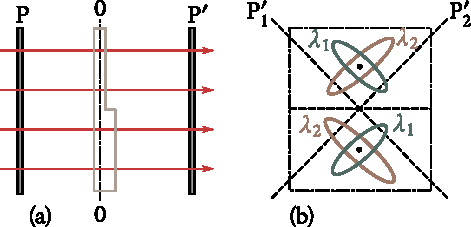
\includegraphics[scale=0.95]{figures/ch_19/fig_19_18.pdf}
		% \caption[]{}
        \caption[]{(a) A plate placed between polarizers. The bottom half of the plate is thicker than the top one. The light passing through the plate contains radiation of only two wavelengths $\lambda_1$ and $\lambda_2$. (b) View from the side of polarizer P$'$. The light components will be elliptically polarized.}
		\label{fig:19_18}
	\end{center}
	\vspace{-0.8cm}
\end{figure}

The phase difference $\delta$ depends on the plate thickness.
Hence, if a doubly refracting transparent plate placed between polarizers has a different thickness at different places, the latter when observed from the side of polarizer P$'$ will seem to be coloured differently.
When polarizer P$'$ is rotated, these colours change, each of them transforming into its complementary colour.
Let us explain this by the following example. Figure \ref{fig:19_18}a shows a plate placed between polarizers.
The bottom half of the plate is thicker than the top one.
Assume that the light passing through the plate contains radiation of only two wavelengths $\lambda_1$ and $\lambda_2$.
Figure \ref{fig:19_18}b gives a ``view'' from
the side of polarizer P$'$.
At the exit from the crystal plate, each of the light components will, generally speaking, be elliptically polarized.
The orientation and the eccentricity of the ellipses for the wavelengths $\lambda_1$ and $\lambda_2$ , and also for different halves of the plate, will be different.
When the plane of polarizer P$'$ is placed in position P$_1'$, in the light transmitted through P$'$ the wavelength $\lambda_1$ will predominate
in the top half of the plate and the wavelength $\lambda_2$ in the bottom half.
Therefore, the two halves will be coloured differently.
When polarizer P$'$ is placed in position P$_2'$, the colour of the top half will be determined by the light of wavelength $\lambda_2$, and of the
bottom half by the light of wavelength $\lambda_1$.
Thus, when polarizer P$'$ is turned through \SI{90}{\degree}, the two halves of the plate exchange colours, as it were.
It is quite natural that this will occur only at a definite ratio of the thicknesses of the two halves of the plate.

\section{Artificial Double Refraction}\label{sec:19_7}

External action may cause double refraction to appear in transparent amorphous bodies, and also in crystals of the cubic system.
This occurs, in particular, upon the mechanical deformations of bodies.
The difference between the refractive indices of an ordinary and an extraordinary ray is a measure of the appearance of optical anisotropy. Experiments show that this difference is proportional to the stress $\sigma$ at a given point of a body (\ie, to the force per unit area;
see Sec. 2.9 of Vol. I):
\begin{equation}\label{eq:19_19}
	\ab{n}{o} - \ab{n}{e} = k \sigma
\end{equation}

\noindent
($k$ is a proportionality constant depending on the properties of the substance).

\begin{figure}[t]
	\begin{center}
		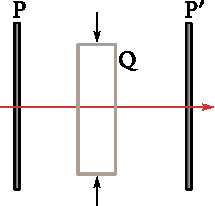
\includegraphics[scale=1]{figures/ch_19/fig_19_19.pdf}
		% \caption[]{}
		\caption[]{Glass plate Q between crossed polarizers P and P$'$. Without glass deformation, there is no transmission of light. Compressing the plate light begins to pass through the system and the pattern observed in the transmitted rays being speckled with coloured fringes. Each fringe corresponds to identically deformed spots on the plate.}
		\label{fig:19_19}
	\end{center}
	\vspace{-0.8cm}
\end{figure}

Let us place glass plate Q between crossed polarizers P and P$'$ (\fig{19_19}).
As long as the glass is not deformed, such a system transmits no light.
If the plate is subjected to compression, light begins to pass through the system, the pattern observed in the transmitted rays being speckled with coloured fringes.
Each fringe corresponds to identically deformed spots on the plate.
Consequently, the distribution of the fringes makes it possible to assess the distribution of the stresses inside the plate.
This underlies the optical method of studying stresses.
A model of a component or structural member made from a transparent isotropic material (for example, from Plexiglas) is placed between crossed polarizers.
The model is subjected to the action of loads similar to those which the article itself will
experience.
The pattern observed in transmitted white light makes it possible to determine the distribution of the stresses and also to estimate their magnitude.

\begin{figure}[t]
	\begin{center}
		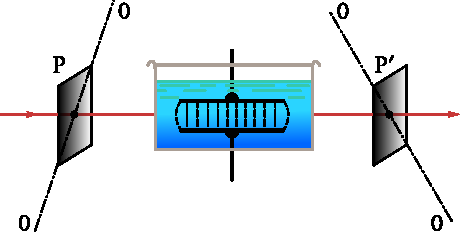
\includegraphics[scale=1]{figures/ch_19/fig_19_20.pdf}
		% \caption[]{}
		\caption[]{Kerr effect in liquids. A Kerr cell is placed between crossed polarizers P and P$'$. The Kerr cell contains liquid into which capacitor plates have been introduced. When a voltage is applied across the plates, a virtually homogeneous electric field is set up between them. Thus, the liquid acquires the properties of a uniaxial crystal with an optical axis oriented along the field.}
		\label{fig:19_20}
	\end{center}
	\vspace{-0.8cm}
\end{figure}

The appearance of double refraction in liquids and amorphous solids under the action of an electric field was discovered by the Scotch physicist John Kerr (1824-1907) in 1875.
This effect was named the \textbf{Kerr effect} after its discoverer.
In 1930, it was also observed in gases.
An arrangement for studying the Kerr effect in liquids is shown schematically in \fig{19_20}.
It consists of a \textbf{Kerr cell} placed between crossed polarizers P and P$'$.
A Kerr cell is a sealed vessel containing a liquid into which capacitor plates have been introduced.
When a voltage is applied across the plates, a virtually homogeneous electric field is set up between them.
Under its action, the liquid acquires the properties of a uniaxial crystal with an optical axis oriented along the field.

The resulting difference between the refractive indices $\ab{n}{o}$ and $\ab{n}{e}$ is proportional to the square of the field strength $E$:
\begin{equation}\label{eq:19_20}
	\ab{n}{o} - \ab{n}{e} = k E^2.
\end{equation}

\noindent
The path difference
\begin{equation*}
	\Delta = (\ab{n}{o} - \ab{n}{e}) l = k l E^2
\end{equation*}

\noindent
appears between the ordinary and extraordinary rays along the path $l$.
The corresponding phase difference is
\begin{equation*}
	\delta = \frac{\Delta}{\lambda_0} 2\pi = 2\pi \frac{k}{\lambda_0} l E^2.
\end{equation*}

\noindent
The latter expression is conventionally written in the form
\begin{equation}\label{eq:19_21}
	\delta = 2\pi B l E^2,
\end{equation}

\noindent
where $B$ is a quantity characteristic of a given substance and known as the \textbf{Kerr constant}.

The Kerr constant depends on the temperature of a substance and on the wavelength of the light.
Among known liquids, nitrobenzene (\ce{C6H5N02}) has the highest Kerr constant.

The Kerr effect is explained by the different polarization of molecules in various directions.
In the absence of a field, the molecules are oriented chaotically, therefore a liquid as a whole displays no anisotropy.
Under the action of a field, the molecules turn so that either their electric dipole moments (in polar molecules) or their directions of maximum polarization (in non-polar molecules) are oriented
in the direction of the field.
As a result, the liquid becomes optically anisotropic.
The thermal motion of the molecules counteracts the orienting action of the field.
This explains the reduction in the Kerr constant with elevation of the temperature.

The time during which the prevailing orientation of the molecules sets in (when the field is switched on) or vanishes (when the field is switched off) is about \SI{e-10}{s}.
Therefore, a Kerr cell placed between crossed polarizers can be used as a virtually inertialess light shutter.
In the absence of a voltage across the capacitor plates, the shutter will be closed.
When the voltage is switched on, the shutter transmits a considerable part of the light falling on the first polarizer.

\section{Rotation of Polarization Plane}\label{sec:19_8}

\textbf{Natural Rotation.}
Some substances known as optically active ones have the ability of causing rotation of the plane of polarization of plane-polarized light passing through them.
Such substances include crystalline bodies (for example, quartz, cinnabar), pure liquids (turpentine, nicotine), and solutions of optically active substances in inactive solvents (aqueous solutions of sugar, tartaric acid, etc.).

Crystalline substances rotate the plane of polarization to the greatest extent when the light propagates along the optical axis of the crystal.
The angle of rotation $\varphi$ is proportional to the path $l$ travelled by a ray in the crystal:
\begin{equation}\label{eq:19_22}
	\varphi = \alpha l.
\end{equation}

\noindent
The coefficient $\alpha$ is called the \textbf{rotational constant}.
It depends on the wavelength (dispersion of the ability to rotate).

In solutions, the angle of rotation of the plane of polarization is proportional to the path of the light in the solution and to the concentration of the active substance, $c$:
\begin{equation}\label{eq:19_23}
	\varphi = [\alpha] c l.
\end{equation}

\noindent
Here. $[\alpha]$ is a quantity called the \textbf{specific rotational constant}.

Depending on the direction of rotation of the polarization plane, optically active substances are divided into \textbf{right-hand} and \textbf{left-hand} ones.
The direction of rotation (relative to a ray) does not depend on the direction of the ray.
Consequently, if a ray that has passed through an optically active crystal along its optical axis is
reflected by a mirror and made to pass through the crystal again in the opposite direction, then the initial position of the polarization plane is restored.

All optically active substances exist in two varieties---right-hand and left-hand.
There exist right-hand and left-hand quartz, right-hand and left-hand sugar, etc.
The molecules or crystals of one variety are a mirror image of the molecules or crystals of the other one (\fig{19_21}).
The symbols C, X, Y, Z, and T stand for atoms or
groups of atoms (radicals) differing from one another.
Molecule (b) is a mirror image of molecule (a).
If we look at the tetrahedron depicted in \fig{19_21} along the direction CX, then in clockwise circumvention we shall encounter the sequence ZYTZ for molecule (a) and ZTYZ for molecule (b).
The same is observed for any of the directions CY, CZ, and CT.
The alternation of the radicals X, Y, Z, T in molecule (b) is the opposite of their alternation in molecule (a).
Consequently, if, for example, a substance formed of molecules (a) is right-hand, then one formed of molecules (b) is left-hand.

\begin{figure}[t]
	\begin{center}
		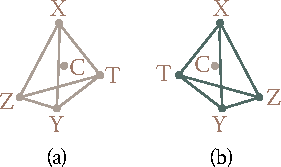
\includegraphics[scale=1]{figures/ch_19/fig_19_21.pdf}
		% \caption[]{}
        \caption[]{Optically active substances exist in two varieties: right-hand and left-hand. The molecules or crystals of a right-hand substance are a mirror image of the molecules or crystals of the left-hand. The symbols C, X, Y, Z, and T stand for atoms or groups of atoms (radicals) differing from one another. Molecule (b) is a mirror image of molecule (a).}
		\label{fig:19_21}
	\end{center}
	\vspace{-0.8cm}
\end{figure}

If we place an optically active substance (a crystal of quartz, a transparent tray with a sugar solution, etc.) between two crossed polarizers, then the field of vision becomes bright.
To get darkness again, one of the polarizers has to be rotated through the angle $\varphi$ determined by expression \eqref{eq:19_22} or \eqref{eq:19_23}.
When a solution is used, we can determine its concentration $c$ by \eqn{19_23} if we know the specific rotational constant $[\alpha]$ of the given substance and the length $l$ and have measured the angle of rotation $\varphi$.
This way of determining the concentration is used in the production of various substances, in particular in the sugar industry (the corresponding instrument is called a saccharimeter).

\textbf{Magnetic Rotation of the Polarization Plane.}
Optically inactive substances acquire the ability of rotating the plane of polarization under the action of a magnetic field.
This phenomenon was discovered by Michael Faraday and is therefore sometimes called the \textbf{Faraday effect}.
It is observed only when light propagates along the direction of magnetization.
Therefore, to observe the Faraday effect, holes are drilled in the pole shoes of an electromagnet, and a light ray is passed through them.
The substance being studied is placed between the poles of the electromagnet.

The angle of rotation of the polarization plane $\varphi$ is proportional to the distance $l$ travelled by the light in the substance and to the
magnetization of the latter.
The magnetization, in turn, is proportional to the magnetic field strength H [see \eqn{7_14}].
We can therefore write that
\begin{equation}\label{eq:19_24}
	\varphi = V l H.
\end{equation}

\noindent
The coefficient $V$ is known as the \textbf{Verdet constant} or the \textbf{specific magnetic
rotation}.
The constant $V$, like the rotational constant $\alpha$, depends on the wavelength.

The direction of rotation is determined by the direction of the magnetic field.
The sign of rotation does not depend on the direction of the ray.
Therefore, if we reflect the ray from a mirror and make it pass through the magnetized substance again in the opposite direction, the rotation of the plane of polarization will double.

The magnetic rotation of the polarization plane is due to the precession of the electron orbits (see \sect{7_7}) produced under the action of the magnetic field.

Optically active substances when acted upon by a magnetic field acquire an additional ability of rotating the plane of polarization that is added to their natural ability.
